% Options for packages loaded elsewhere
\PassOptionsToPackage{unicode}{hyperref}
\PassOptionsToPackage{hyphens}{url}
%
\documentclass[
  ignorenonframetext,
  serif,
  professionalfont,
  usenames,
  dvipsnames,
  aspectratio = 169]{beamer}
\usepackage{pgfpages}
\setbeamertemplate{caption}[numbered]
\setbeamertemplate{caption label separator}{: }
\setbeamercolor{caption name}{fg=normal text.fg}
\beamertemplatenavigationsymbolsempty
% Prevent slide breaks in the middle of a paragraph
\widowpenalties 1 10000
\raggedbottom
\setbeamertemplate{part page}{
  \centering
  \begin{beamercolorbox}[sep=16pt,center]{part title}
    \usebeamerfont{part title}\insertpart\par
  \end{beamercolorbox}
}
\setbeamertemplate{section page}{
  \centering
  \begin{beamercolorbox}[sep=12pt,center]{part title}
    \usebeamerfont{section title}\insertsection\par
  \end{beamercolorbox}
}
\setbeamertemplate{subsection page}{
  \centering
  \begin{beamercolorbox}[sep=8pt,center]{part title}
    \usebeamerfont{subsection title}\insertsubsection\par
  \end{beamercolorbox}
}
\AtBeginPart{
  \frame{\partpage}
}
\AtBeginSection{
  \ifbibliography
  \else
    \frame{\sectionpage}
  \fi
}
\AtBeginSubsection{
  \frame{\subsectionpage}
}
\usepackage{amsmath,amssymb}
\usepackage{lmodern}
\usepackage{iftex}
\ifPDFTeX
  \usepackage[T1]{fontenc}
  \usepackage[utf8]{inputenc}
  \usepackage{textcomp} % provide euro and other symbols
\else % if luatex or xetex
  \usepackage{unicode-math}
  \defaultfontfeatures{Scale=MatchLowercase}
  \defaultfontfeatures[\rmfamily]{Ligatures=TeX,Scale=1}
\fi
% Use upquote if available, for straight quotes in verbatim environments
\IfFileExists{upquote.sty}{\usepackage{upquote}}{}
\IfFileExists{microtype.sty}{% use microtype if available
  \usepackage[]{microtype}
  \UseMicrotypeSet[protrusion]{basicmath} % disable protrusion for tt fonts
}{}
\makeatletter
\@ifundefined{KOMAClassName}{% if non-KOMA class
  \IfFileExists{parskip.sty}{%
    \usepackage{parskip}
  }{% else
    \setlength{\parindent}{0pt}
    \setlength{\parskip}{6pt plus 2pt minus 1pt}}
}{% if KOMA class
  \KOMAoptions{parskip=half}}
\makeatother
\usepackage{xcolor}
\newif\ifbibliography
\usepackage{longtable,booktabs,array}
\usepackage{calc} % for calculating minipage widths
\usepackage{caption}
% Make caption package work with longtable
\makeatletter
\def\fnum@table{\tablename~\thetable}
\makeatother
\usepackage{graphicx}
\makeatletter
\def\maxwidth{\ifdim\Gin@nat@width>\linewidth\linewidth\else\Gin@nat@width\fi}
\def\maxheight{\ifdim\Gin@nat@height>\textheight\textheight\else\Gin@nat@height\fi}
\makeatother
% Scale images if necessary, so that they will not overflow the page
% margins by default, and it is still possible to overwrite the defaults
% using explicit options in \includegraphics[width, height, ...]{}
\setkeys{Gin}{width=\maxwidth,height=\maxheight,keepaspectratio}
% Set default figure placement to htbp
\makeatletter
\def\fps@figure{htbp}
\makeatother
\setlength{\emergencystretch}{3em} % prevent overfull lines
\providecommand{\tightlist}{%
  \setlength{\itemsep}{0pt}\setlength{\parskip}{0pt}}
\setcounter{secnumdepth}{-\maxdimen} % remove section numbering
% Definição do esquema de cores:
% 1. UFPR - Azul com cinza.
% 2. DEST - Roxo com cinza.
% 3. LEG - Laranjado com cinza.
\def\mycolorscheme{1}

% Caminho para a imagem de fundo com aspecto 16x9.
% \def\pathtobg{config/ufpr-fachada-baixo-1.jpg}
% \def\pathtobg{config/ufpr-fundo.jpg}
% \def\pathtobg{config/ufpr-fundo.jpg}
\def\pathtobg{./config/ufpr-fundo-16x9.jpg}

% \providecommand{\tightlist}{%
%   \setlength{\itemsep}{0pt}\setlength{\parskip}{0pt}}
% ATTENTION: Redefine o comando acima que é definido pelo template.
% \renewcommand{\tightlist}{}
\renewcommand{\tightlist}{%
  \setlength{\itemsep}{0\baselineskip}
  \setlength{\parskip}{0.25\baselineskip}
}

% Logo na capa.
\titlegraphic{
  %\vspace{-1em}
  %\includegraphics[height=1.2cm]{config/dest-texto-2.png}\hspace{1em}
  %\includegraphics[height=1.8cm]{config/dsbd-logo-2x2.png}\hspace{1em}
  
\includegraphics[height=1.8cm]{config/ufpr-transparent-600px.png}
}
%-----------------------------------------------------------------------

% Palladio.
% \usepackage[sc]{mathpazo}
% \linespread{1.05}         % Palladio needs more leading (space between lines)
% \usepackage[T1]{fontenc}

% Kurier.
% \usepackage[light, condensed, math]{kurier}
% \usepackage[T1]{fontenc}

% Iwona.
% \usepackage[math, light, condensed]{iwona}

% \usepackage{cmbright}
% \usepackage[charter]{mathdesign}
% \usepackage{palatino}

% Roboto (with Iwona for maths).
% \usepackage[math]{iwona}
% \usepackage[sfdefault, light, condensed]{roboto}

% Source Sans Pro (with Iwona for maths).
% \usepackage[math]{iwona}
% \usepackage[default, light]{sourcesanspro}

% Lato (with Iwona for maths).
% \usepackage[math]{iwona}
% \usepackage[default]{lato}

% Fira Sans (with Iwona for maths).
\usepackage[math, light]{iwona}
\usepackage[sfdefault,light]{FiraSans} %% option 'sfdefault' activates Fira Sans as the default text font
\usepackage[T1]{fontenc}
\renewcommand*\oldstylenums[1]{{\firaoldstyle #1}}

% Font for code. ----------------------------
% \usepackage[scaled=.75]{beramono}
\usepackage{inconsolata}

% ATTENTION: needs complile with xelatex: `$ xelatex file.tex`
% \usepackage{fontspec}
% \setmonofont{M+ 1m}
% \setmonofont{M+ 1mn}
% \setmonofont{M+ 2m}

%-----------------------------------------------------------------------

% \usepackage{lmodern}
\usepackage{amssymb, amsmath}
\usepackage[makeroom]{cancel}
% \usepackage{ifxetex, ifluatex}
\usepackage{fixltx2e} % provides \textsubscript
\usepackage[utf8]{inputenc}
\usepackage[shorthands=off,main=brazil]{babel}
\usepackage{graphicx}
\usepackage{xcolor}
\usepackage{setspace}
\usepackage{comment}
\usepackage{icomma}

%-----------------------------------------------------------------------
% Algumas configurações.

\setlength{\parindent}{0pt}
\setlength{\parskip}{6pt plus 2pt minus 1pt}
\setlength{\emergencystretch}{3em}  % prevent overfull lines
% \providecommand{\tightlist}{%
%   \setlength{\itemsep}{0pt}\setlength{\parskip}{0pt}}
\setcounter{secnumdepth}{0}

% Espaço vertical para o ambiente `quote`.
\let\oldquote\quote
\let\oldendquote\endquote
\renewenvironment{quote}{%
  \vspace{1em}\oldquote}{%
  \oldendquote\vspace{1em}}

%-----------------------------------------------------------------------
% Espaçamento entre items para itemize, enumerate e description.

% % itemize.
% \let\itemopen\itemize
% \let\itemclose\enditemize
% \renewenvironment{itemize}{%
%   \itemopen\addtolength{\itemsep}{0.25\baselineskip}}{\itemclose}
%
% % enumerate.
% \let\enumopen\enumerate
% \let\enumclose\endenumerate
% \renewenvironment{enumerate}{%
%   \enumopen\addtolength{\itemsep}{0.25\baselineskip}}{\enumclose}
%
% % description.
% \let\descopen\description
% \let\descclose\enddescription
% \renewenvironment{description}{%
%   \descopen\addtolength{\itemsep}{0.25\baselineskip}}{\descclose}

%-----------------------------------------------------------------------

% \usepackage[hang]{caption}
\usepackage{caption}
\captionsetup{font=footnotesize,
  labelfont={color=mycolor1, footnotesize},
  labelsep=period}

% \providecommand{\tightlist}{%
%   \setlength{\itemsep}{0pt}\setlength{\parskip}{0pt}}

%-----------------------------------------------------------------------

\usepackage{tikz}

% \def\pathtobg{/home/walmes/Projects/templates/COMMON/ufpr-fundo.jpg}
% \def\pathtobg{/home/walmes/Projects/templates/COMMON/ufpr-fundo-16x9.jpg}
% \def\pathtobg{/home/walmes/Projects/templates/COMMON/ufpr-fachada-dir-1.jpg}
% \def\pathtobg{/home/walmes/Projects/templates/COMMON/ufpr-fachada-esq-1.jpg}
% \def\pathtobg{/home/walmes/Projects/templates/COMMON/ufpr-perto-1.jpg}
% \def\pathtobg{/home/walmes/Projects/templates/COMMON/ufpr-fachada-baixo-1.jpg}

\ifx\pathtobg\undefined
\else
  \usebackgroundtemplate{
    \tikz[overlay, remember picture]
    \node[% opacity=0.3,
          at=(current page.south east),
          anchor=south east,
          inner sep=0pt] {
            \includegraphics[height=\paperheight, width=\paperwidth]{\pathtobg}};
  }
\fi

%-----------------------------------------------------------------------
% Definições de esquema de cores.

\ifx\mycolorscheme\undefined
  % UFPR.
  % http://www.color-hex.com/color-palette/2018
  \definecolor{mycolor1}{HTML}{015c93} % Título.
  \definecolor{mycolor2}{HTML}{363435} % Texto.
  \definecolor{mycolor3}{HTML}{015c93} % Estrutura.
  \definecolor{mycolor4}{HTML}{015c93} % Links.
  \definecolor{mycolor5}{HTML}{CECAC5} % Preenchimentos.
\else
  \if\mycolorscheme1
    % UFPR.
    \definecolor{mycolor1}{HTML}{015c93} % Título.
    \definecolor{mycolor2}{HTML}{363435} % Texto.
    \definecolor{mycolor3}{HTML}{015c93} % Estrutura.
    \definecolor{mycolor4}{HTML}{015c93} % Links.
    \definecolor{mycolor5}{HTML}{CECAC5} % Preenchimentos.
  \fi
  \if\mycolorscheme2
    % DEST.
    \definecolor{mycolor1}{HTML}{2a0e72} % Título.
    \definecolor{mycolor2}{HTML}{202E35} % Texto.
    \definecolor{mycolor3}{HTML}{2a0e72} % Estrutura.
    % \definecolor{mycolor3}{HTML}{8072a3} % Estrutura.
    \definecolor{mycolor4}{HTML}{2a0e72} % Links.
    % \definecolor{mycolor4}{HTML}{bfb9d1} % Links.
    % \definecolor{mycolor5}{HTML}{AEA79F} % Preenchimentos.
    \definecolor{mycolor5}{HTML}{CECAC5} % Preenchimentos.
  \fi
  \if\mycolorscheme3
    % LEG.
    \definecolor{mycolor2}{HTML}{363435} % Texto.
    % \definecolor{mycolor1}{HTML}{ff8000} % Título.
    % \definecolor{mycolor3}{HTML}{ff8000} % Estrutura.
    % \definecolor{mycolor4}{HTML}{ff8000} % Links.
    % \definecolor{mycolor1}{HTML}{E57300} % Título.
    % \definecolor{mycolor3}{HTML}{E57300} % Estrutura.
    % \definecolor{mycolor4}{HTML}{E57300} % Links.
    \definecolor{mycolor1}{HTML}{F67014} % Título.
    \definecolor{mycolor3}{HTML}{F67014} % Estrutura.
    \definecolor{mycolor4}{HTML}{F67014} % Links.
    % \definecolor{mycolor1}{HTML}{FE5C23} % Título.
    % \definecolor{mycolor3}{HTML}{FE5C23} % Estrutura.
    % \definecolor{mycolor4}{HTML}{FE5C23} % Links.
    \definecolor{mycolor5}{HTML}{222222} % Preenchimentos.
    \definecolor{mycolor5}{HTML}{383838} % Preenchimentos.
  \fi
\fi

\hypersetup{
  colorlinks=true,
  linkcolor=mycolor4,
  urlcolor=mycolor1,
  citecolor=mycolor1
}

%-----------------------------------------------------------------------
% ATTENTION: http://www.cpt.univ-mrs.fr/~masson/latex/Beamer-appearance-cheat-sheet.pdf

\usetheme{Boadilla}
\usecolortheme{default}

% \setbeamersize{text margin left=7mm, text margin right=7mm}
% \setbeamertemplate{frametitle}[default][left, leftskip=3mm]
% \addtobeamertemplate{frametitle}{\vspace{0.5em}}{}

\setbeamertemplate{caption}[numbered]
\setbeamertemplate{section in toc}[sections numbered]
\setbeamertemplate{subsection in toc}[subsections numbered]
\setbeamertemplate{sections/subsections in toc}[ball]{}
\setbeamertemplate{sections in toc}[ball]
\setbeamercolor{section number projected}{bg=mycolor1, fg=white}
\setbeamertemplate{blocks}[rounded]
\setbeamertemplate{navigation symbols}{}
\setbeamertemplate{frametitle continuation}{\gdef\beamer@frametitle{}}
% \setbeamertemplate{frametitle}[default][center]
% \setbeamertemplate{footline}[frame number]

\setbeamertemplate{enumerate items}[default]
\setbeamertemplate{itemize items}{\scriptsize\raise1.25pt\hbox{\donotcoloroutermaths$\blacktriangleright$}}

% Blocos.
% \addtobeamertemplate{block begin}{\vskip -\bigskipamount}{}
% \addtobeamertemplate{block end}{}{\vskip -\bigskipamount}
\addtobeamertemplate{block begin}{\vspace{0.5em}}{}
\addtobeamertemplate{block end}{}{\vspace{0.5em}}


% Rodapé.
\setbeamercolor{title in head/foot}{parent=subsection in head/foot}
\setbeamercolor{author in head/foot}{bg=mycolor4, fg=white}
\setbeamercolor{date in head/foot}{parent=subsection in head/foot, fg=mycolor3}

% Cabeçalho.
\setbeamercolor{section in head/foot}{bg=mycolor2, fg=mycolor4}
\setbeamercolor{subsection in head/foot}{bg=mycolor2, fg=white}

\setbeamercolor{title}{fg=mycolor1}       % Título dos slides.
\setbeamercolor{titlelike}{fg=title}
\setbeamercolor{subtitle}{fg=mycolor2}    % Subtítulo.
\setbeamercolor{institute in head/foot}{parent=palette primary} % Instituição.
\setbeamercolor{frametitle}{fg=mycolor1}  % De quadro.
\setbeamercolor{structure}{fg=mycolor3}   % Listas e rodapé.
\setbeamercolor{item projected}{bg=mycolor2}
\setbeamercolor{block title}{bg=mycolor5, fg=mycolor2}
\setbeamercolor{normal text}{fg=mycolor2} % Texto.
\setbeamercolor{caption name}{fg=normal text.fg}
% \setbeamercolor{footlinecolor}{fg=mycolor2, bg=mycolor5}
% \setbeamercolor{section in head/foot}{fg=mycolor2, bg=mycolor5}
\setbeamercolor{author in head/foot}{fg=white, bg=mycolor1}
\setbeamercolor{section in foot}{fg=mycolor4, bg=mycolor5}
\setbeamercolor{date in foot}{fg=mycolor4, bg=mycolor5}
\setbeamercolor{block title}{fg=white, bg=mycolor1}
\setbeamercolor{block body}{fg=black, bg=white!80!gray}
\setbeamercolor{block body}{fg=black, bg=white!80!gray}

% To remove empty brackets of \institution.
\makeatletter
\setbeamertemplate{footline}{
  \leavevmode%
  \hbox{%
    \begin{beamercolorbox}[
      wd=0.3\paperwidth, ht=2.25ex, dp=1ex, right]{author in head/foot}%
      \usebeamerfont{author in head/foot}\insertshortauthor{}\hspace*{1ex}
    \end{beamercolorbox}%
    \begin{beamercolorbox}[
      wd=0.6\paperwidth, ht=2.25ex, dp=1ex, left]{section in foot}%
      \usebeamerfont{title in head/foot}\hspace*{1ex}\insertshorttitle{}
      % \usebeamerfont{title in head/foot}\hspace*{1ex}\insertframetitle{}
    \end{beamercolorbox}%
    \begin{beamercolorbox}[
      wd=0.1\paperwidth, ht=2.25ex, dp=1ex, right]{date in foot}%
      \insertframenumber{}\hspace*{2ex}
    \end{beamercolorbox}
  }%
  \vskip0pt%
}
\makeatother

%-----------------------------------------------------------------------

% \usepackage{hyphenat}
\usepackage{changepage}

% Slide para o título das seções.
\AtBeginSection[]{
  \begin{frame}
    % \vfill
    \vspace{4cm}
    % \centering
    % \begin{beamercolorbox}[sep = 8pt, center, shadow = true, rounded = true]{title}
    \begin{beamercolorbox}{title}
      \begin{columns}
        \column{0.7\linewidth}
        {\LARGE\textbf \insertsectionhead}
      \end{columns}
    \end{beamercolorbox}
    \vfill
  \end{frame}
}

%-----------------------------------------------------------------------
%---- preamble-chunk.tex -----------------------------------------------

% Knitr.

% ATTENTION: this needs `\usepackage{xcolor}'.
\definecolor{color_line}{HTML}{333333}
\definecolor{color_back}{HTML}{DDDDDD}
% \definecolor{color_back}{HTML}{FF0000}

% ATTENTION: usa o fancyvrb.
% https://ctan.math.illinois.edu/macros/latex/contrib/fancyvrb/doc/fancyvrb-doc.pdf
% R input.
\usepackage{tcolorbox}
\ifcsmacro{Highlighting}{
  % Statment if it exists. ------------------
  \DefineVerbatimEnvironment{Highlighting}{Verbatim}{
    % frame=lines,     % Linha superior e inferior.
    % framerule=0.5pt, % Espessura da linha.
    framesep=2ex,    % Distância da linha para o texto.
    % rulecolor=\color{color_line},
    % numbers=right,
    fontsize=\footnotesize, % Tamanho da fonte.
    baselinestretch=0.8,    % Espaçamento entre linhas.
    commandchars=\\\{\}}
  % Margens do ambiente `Shaded'.
  % \fvset{listparameters={\setlength{\topsep}{-1em}}}
  % \renewenvironment{Shaded}{\vspace{-1ex}}{\vspace{-2ex}}
  \renewenvironment{Shaded}{
    \vspace{2pt}
    \begin{tcolorbox}[
      boxrule=0pt,      % Espessura do contorno.
      colframe=gray!10, % Cor do contorno.
      colback=gray!10,  % Cor de fundo da caixa.
      arc=1em,          % Raio para contornos arredondados.
      sharp corners,
      boxsep=0.5em,     % Margem interna.
      left=3pt, right=3pt, top=3pt, bottom=3pt, % Margens internas.
      grow to left by=0mm,
      grow to right by=6pt,
      ]
    }{
    \end{tcolorbox}
    \vspace{-3pt}
    }
  }{
  % Statment if it not exists. --------------
}

% R output e todo `verbatim'.
\makeatletter
\def\verbatim@font{\linespread{0.8}\ttfamily\footnotesize}
%\makeatother

% Cor de fundo e margens do `verbatim'.
\let\oldv\verbatim
\let\oldendv\endverbatim

\def\verbatim{%
  \par\setbox0\vbox\bgroup % Abre grupo.
  %\vspace{-5px}            % Reduz margem superior.
  \oldv                    % Chama abertura do verbatim.
}
\def\endverbatim{%
  \oldendv                 % Chama encerramento do verbatim.
  %\vspace{0cm}           % Controla margem inferior.
  \egroup%\fboxsep5px      % Fecha grupo.
  \noindent{{\usebox0}}\par
}

%-----------------------------------------------------------------------
%---- preamble-commands.tex --------------------------------------------

% Para fazer texto em duas colunas.
\newcommand{\mytwocolumns}[4]{
  % #1: Line width fraction for the left column , e.g. 0.5.
  % #2: Line width fraction for the right column.
  % #3: Content for the left column.
  % #4: Content for the right column.
  \begin{columns}[c]
    \begin{column}{#1\linewidth} %----------- left.
      #3
    \end{column} %--------------------------- left.
    \begin{column}{#2\linewidth} %----------- right.
      #4
    \end{column} %--------------------------- right.
  \end{columns}
}

%-----------------------------------------------------------------------
% Para fazer duas colunas no Rmd.

% Center vertical align.
\def\beginAHalfColumn{\begin{minipage}{0.49\textwidth}}%
\def\beginAlmostHalfColumn{\begin{minipage}{0.45\textwidth}}%
\def\beginAQuarterColumn{\begin{minipage}{0.23\textwidth}}%
\def\beginThreeQuartersColumn{\begin{minipage}{0.72\textwidth}}%
\def\beginAThirdColumn{\begin{minipage}{0.31\textwidth}}%
\def\beginTwoThirdsColumn{\begin{minipage}{0.64\textwidth}}%
\def\endColumns{\end{minipage}}%

% Top vertical align.
\def\beginAHalfColumnT{\begin{minipage}[t]{0.49\textwidth}}%
\def\beginAlmostHalfColumnT{\begin{minipage}[t]{0.45\textwidth}}%
\def\beginAQuarterColumnT{\begin{minipage}[t]{0.23\textwidth}}%
\def\beginThreeQuartersColumnT{\begin{minipage}[t]{0.72\textwidth}}%
\def\beginAThirdColumnT{\begin{minipage}[t]{0.31\textwidth}}%
\def\beginTwoThirdsColumnT{\begin{minipage}[t]{0.64\textwidth}}%

%---------------------------------------------------------------------
% Ambientes para frases como e sem imagem.

\newcommand{\myquote}[3]{
  % #1: caminho para a imagem.
  % #2: a frase/quotation.
  % #3: o autor.
  \begin{center}
    \begin{minipage}[c]{0.19\linewidth}
      \begin{center}
        \includegraphics[height=2.5cm]{#1}
      \end{center}
    \end{minipage}
    \begin{minipage}[c]{0.7\linewidth}
      \begin{flushright}
        \textit{#2}
        \vspace{1ex}

        -- #3
      \end{flushright}
    \end{minipage}
  \end{center}
}

\newcommand{\myphrase}[2]{
  % #1: a frase/quotation.
  % #2: o autor.
  \begin{center}
    \begin{minipage}[c]{0.19\linewidth}
    \end{minipage}
    \begin{minipage}[c]{0.7\linewidth}
      \begin{flushright}
        \textit{#1}
        \vspace{1ex}

        -- #2
      \end{flushright}
    \end{minipage}
  \end{center}
}

%-----------------------------------------------------------------------
% Comandos para texto em destaque.

% \newcommand{\hi}[1]{%
%   \textcolor{ubuntu_orange}{#1}\xspace
% }

\usepackage{xspace}

% URLs com letra miuda.
\newcommand{\myurl}[1]{%
  {\tiny \url{#1}}\xspace
}

% Botões.
\newcommand{\btn}[1]{%
  \beamergotobutton{#1}\xspace
}

% Texto grande centralizado.
\newcommand{\centertitle}[1]{%
  \begin{center}
    {\LARGE \bfseries \hi{#1}}
  \end{center}
}

%-----------------------------------------------------------------------
\ifLuaTeX
  \usepackage{selnolig}  % disable illegal ligatures
\fi
\IfFileExists{bookmark.sty}{\usepackage{bookmark}}{\usepackage{hyperref}}
\IfFileExists{xurl.sty}{\usepackage{xurl}}{} % add URL line breaks if available
\urlstyle{same} % disable monospaced font for URLs
\hypersetup{
  pdfauthor={Prof.~Me. Lineu Alberto Cavazani de Freitas},
  hidelinks,
  pdfcreator={LaTeX via pandoc}}

\title{\textbf{Análise exploratória III}}
\subtitle{Análises bivariadas}
\author{Prof.~Me. Lineu Alberto Cavazani de Freitas}
\date{}
\institute{\textbf{CE003 – Estatística II}\\
\strut \\
Departamento de Estatística\\
Laboratório de Estatística e Geoinformação}

\begin{document}
\frame{\titlepage}

\begin{frame}{Análise exploratória bivariada}
\protect\hypertarget{anuxe1lise-exploratuxf3ria-bivariada}{}
\beginAHalfColumn

\begin{itemize}
\item
  Em alguns casos podemos estar interessados na análise de duas
  variáveis simultaneamente.
\item
  O objetivo é investigar a relação de \textbf{associação} entre as
  variáveis.
\item
  Tabelas, gráficos e coeficientes específicos para relação entre
  variáveis podem ser usados.
\end{itemize}

\endColumns
\beginAHalfColumn

\begin{itemize}
\item
  Tal como nas análises univariadas, as escolhas dependem dos tipos de
  variáveis.
\item
  Considerando variáveis aos pares, as combinações podem ser:

  \begin{itemize}
  \tightlist
  \item
    Qualitativa x qualitativa.
  \item
    Quantitativa x quantitativa.
  \item
    Quantitativa x qualitativa.
  \end{itemize}
\end{itemize}

\endColumns
\end{frame}

\hypertarget{anuxe1lise-bivariada-para-variuxe1veis-qualitativas}{%
\section{Análise bivariada para variáveis
qualitativas}\label{anuxe1lise-bivariada-para-variuxe1veis-qualitativas}}

\begin{frame}{Análise bivariada para variáveis qualitativas}
\protect\hypertarget{anuxe1lise-bivariada-para-variuxe1veis-qualitativas-1}{}
\begin{itemize}
\item
  Neste tipo de situação avaliamos a \textbf{frequência} de observações
  para cada \textbf{combinação} de níveis das duas variáveis.
\item
  Podem ser usadas \textbf{tabelas de frequências cruzadas}, também
  chamadas de \textbf{tabelas de dupla entrada}.
\item
  Também é possível representar as frequências por meio de
  \textbf{recursos gráficos}.
\end{itemize}
\end{frame}

\begin{frame}{Tabelas de frequências cruzadas}
\protect\hypertarget{tabelas-de-frequuxeancias-cruzadas}{}
\begin{itemize}
\tightlist
\item
  As linhas dizem respeito aos níveis de uma variável.
\item
  As colunas aos níveis da outra variável.
\item
  As células mostram as frequências (absolutas ou relativas).
\item
  As margens mostram as frequências marginais (de apenas uma das duas
  variáveis).
\item
  No caso de frequências relativas podem ser usados os totais linha,
  coluna ou o total geral.
\end{itemize}
\end{frame}

\begin{frame}{Tabelas de frequências cruzadas}
\protect\hypertarget{tabelas-de-frequuxeancias-cruzadas-1}{}
\begin{longtable}[]{@{}lcccccc@{}}
\caption{Tabela de dupla entrada para\ldots{}}\tabularnewline
\toprule()
& f & g & h & i & j & Total \\
\midrule()
\endfirsthead
\toprule()
& f & g & h & i & j & Total \\
\midrule()
\endhead
a & 21 & 12 & 19 & 15 & 22 & 89 \\
b & 16 & 21 & 16 & 28 & 30 & 111 \\
c & 15 & 15 & 22 & 19 & 24 & 95 \\
d & 17 & 22 & 21 & 20 & 27 & 107 \\
e & 20 & 31 & 18 & 17 & 12 & 98 \\
Total & 89 & 101 & 96 & 99 & 115 & 500 \\
\bottomrule()
\end{longtable}
\end{frame}

\begin{frame}{Tabelas de frequências cruzadas}
\protect\hypertarget{tabelas-de-frequuxeancias-cruzadas-2}{}
\begin{longtable}[]{@{}lcccccc@{}}
\caption{Tabela de dupla entrada total linha\ldots{}}\tabularnewline
\toprule()
& f & g & h & i & j & Total \\
\midrule()
\endfirsthead
\toprule()
& f & g & h & i & j & Total \\
\midrule()
\endhead
a & 0.24 & 0.13 & 0.21 & 0.17 & 0.25 & 1 \\
b & 0.14 & 0.19 & 0.14 & 0.25 & 0.27 & 1 \\
c & 0.16 & 0.16 & 0.23 & 0.20 & 0.25 & 1 \\
d & 0.16 & 0.21 & 0.20 & 0.19 & 0.25 & 1 \\
e & 0.20 & 0.32 & 0.18 & 0.17 & 0.12 & 1 \\
Total & 0.90 & 1.00 & 0.97 & 0.98 & 1.14 & 5 \\
\bottomrule()
\end{longtable}
\end{frame}

\begin{frame}{Tabelas de frequências cruzadas}
\protect\hypertarget{tabelas-de-frequuxeancias-cruzadas-3}{}
\begin{longtable}[]{@{}lcccccc@{}}
\caption{Tabela de dupla entrada total coluna\ldots{}}\tabularnewline
\toprule()
& f & g & h & i & j & Total \\
\midrule()
\endfirsthead
\toprule()
& f & g & h & i & j & Total \\
\midrule()
\endhead
a & 0.24 & 0.12 & 0.20 & 0.15 & 0.19 & 0.90 \\
b & 0.18 & 0.21 & 0.17 & 0.28 & 0.26 & 1.10 \\
c & 0.17 & 0.15 & 0.23 & 0.19 & 0.21 & 0.95 \\
d & 0.19 & 0.22 & 0.22 & 0.20 & 0.23 & 1.06 \\
e & 0.22 & 0.31 & 0.19 & 0.17 & 0.10 & 1.00 \\
Total & 1.00 & 1.00 & 1.00 & 1.00 & 1.00 & 5.00 \\
\bottomrule()
\end{longtable}
\end{frame}

\begin{frame}{Tabelas de frequências cruzadas}
\protect\hypertarget{tabelas-de-frequuxeancias-cruzadas-4}{}
\begin{longtable}[]{@{}lcccccc@{}}
\caption{Tabela de dupla entrada total geral\ldots{}}\tabularnewline
\toprule()
& f & g & h & i & j & Total \\
\midrule()
\endfirsthead
\toprule()
& f & g & h & i & j & Total \\
\midrule()
\endhead
a & 0.04 & 0.02 & 0.04 & 0.03 & 0.04 & 0.18 \\
b & 0.03 & 0.04 & 0.03 & 0.06 & 0.06 & 0.22 \\
c & 0.03 & 0.03 & 0.04 & 0.04 & 0.05 & 0.19 \\
d & 0.03 & 0.04 & 0.04 & 0.04 & 0.05 & 0.21 \\
e & 0.04 & 0.06 & 0.04 & 0.03 & 0.02 & 0.20 \\
Total & 0.18 & 0.20 & 0.19 & 0.20 & 0.23 & 1.00 \\
\bottomrule()
\end{longtable}
\end{frame}

\begin{frame}{Análise bivariada para variáveis qualitativas}
\protect\hypertarget{anuxe1lise-bivariada-para-variuxe1veis-qualitativas-2}{}
\beginAHalfColumn

\begin{itemize}
\item
  As frequências cruzadas podem ser representadas por meio de gráficos.
\item
  Variações de gráficos de barras são as opções mais comuns.
\item
  As possibilidades podem usar as frequências absolutas, relativas e
  permitem comparar a composição das variáveis.
\end{itemize}

\endColumns
\beginAHalfColumn

\begin{itemize}
\tightlist
\item
  Gráficos para frequência para duas variáveis qualitativas:

  \begin{itemize}
  \tightlist
  \item
    Gráficos de barras lado a lado.
  \item
    Gráfico de barras empilhadas.
  \item
    Gráficos de barras empilhadas relativo.
  \end{itemize}
\end{itemize}

\endColumns
\end{frame}

\begin{frame}{Gráficos de barras lado a lado}
\protect\hypertarget{gruxe1ficos-de-barras-lado-a-lado}{}
\begin{figure}

{\centering 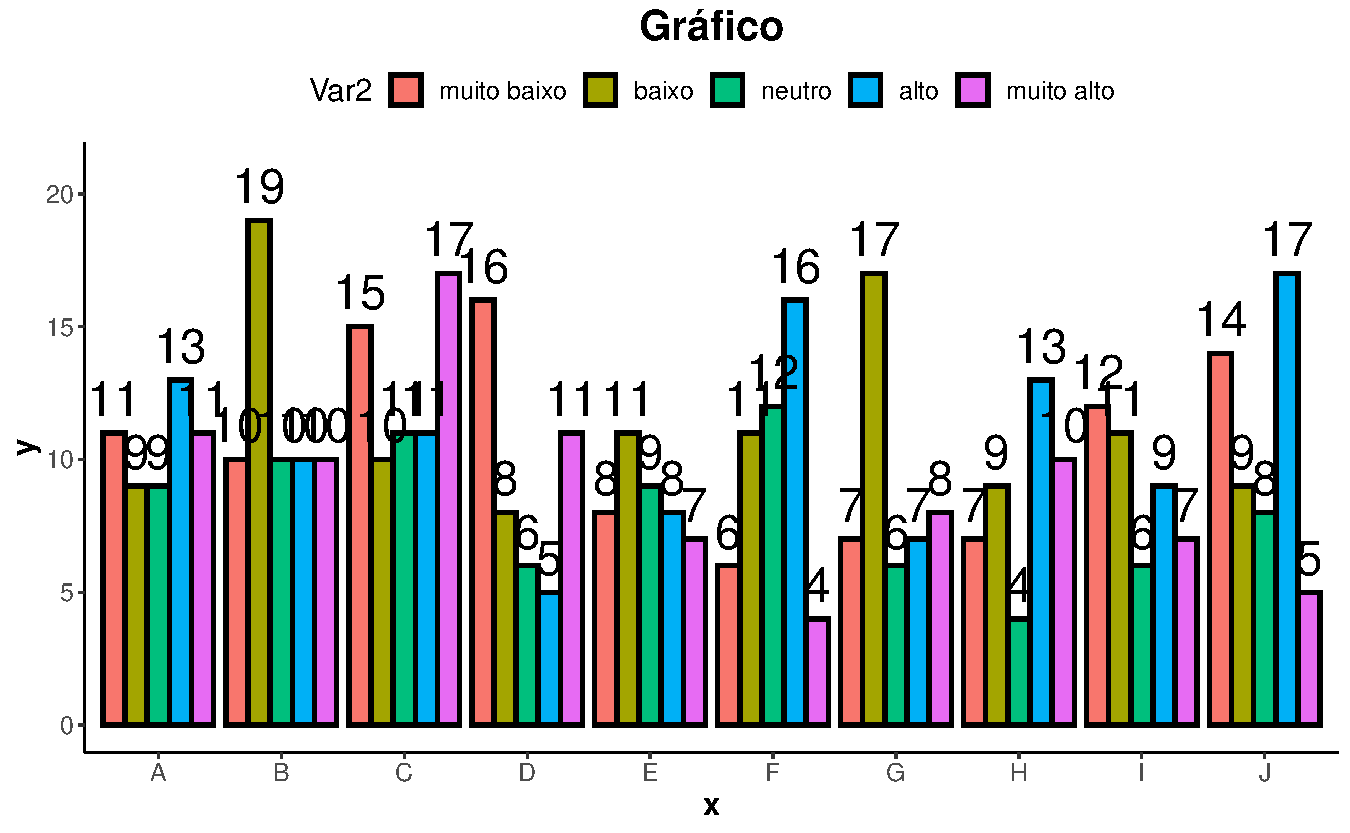
\includegraphics[width=11cm]{202-exploratoria-bivariada_files/figure-beamer/unnamed-chunk-6-1} 

}

\caption{Gráfico de barras lado a lado...}\label{fig:unnamed-chunk-6}
\end{figure}
\end{frame}

\begin{frame}{Gráficos de barras empilhadas}
\protect\hypertarget{gruxe1ficos-de-barras-empilhadas}{}
\begin{figure}

{\centering 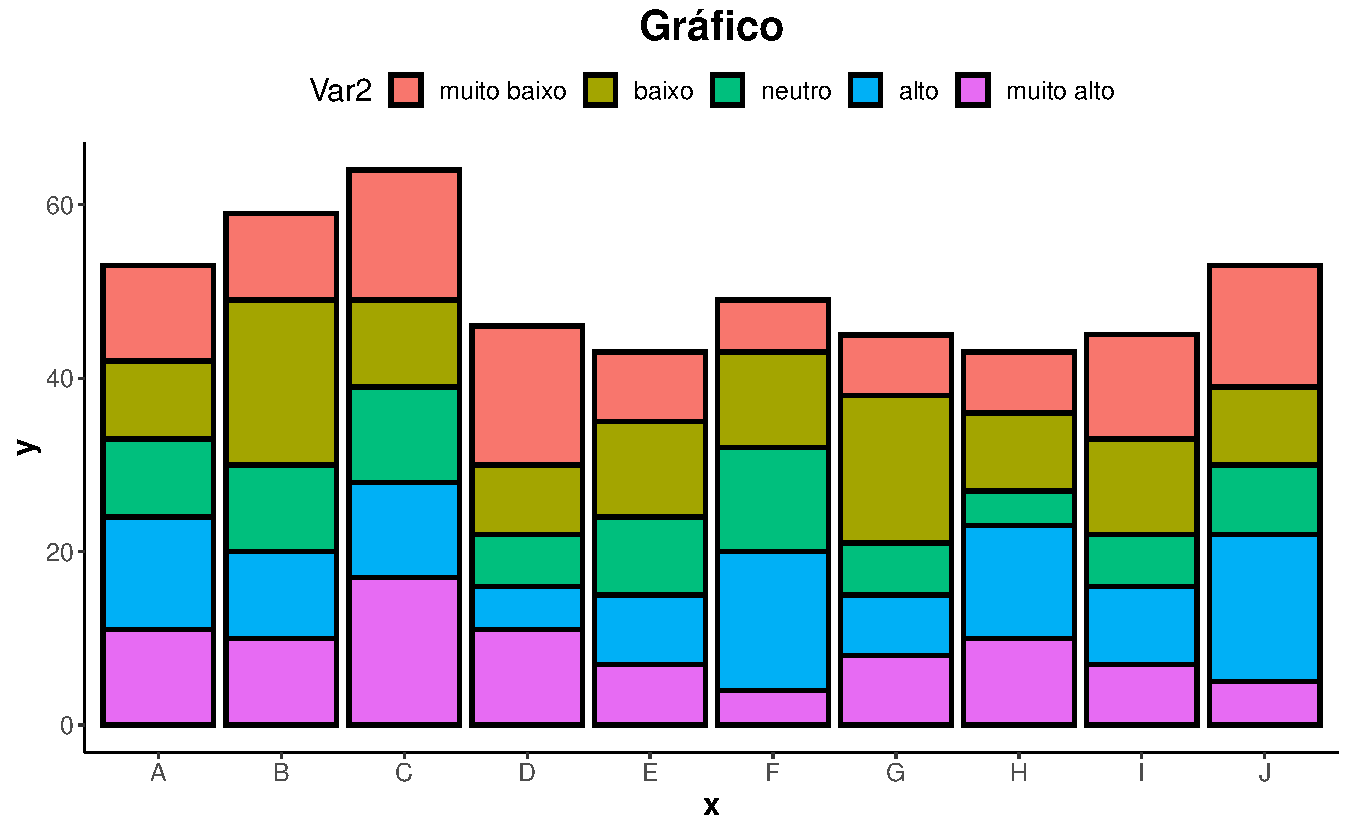
\includegraphics[width=11cm]{202-exploratoria-bivariada_files/figure-beamer/unnamed-chunk-7-1} 

}

\caption{Gráfico de barras empilhadas...}\label{fig:unnamed-chunk-7}
\end{figure}
\end{frame}

\begin{frame}{Gráficos de barras empilhadas relativo}
\protect\hypertarget{gruxe1ficos-de-barras-empilhadas-relativo}{}
\begin{figure}

{\centering 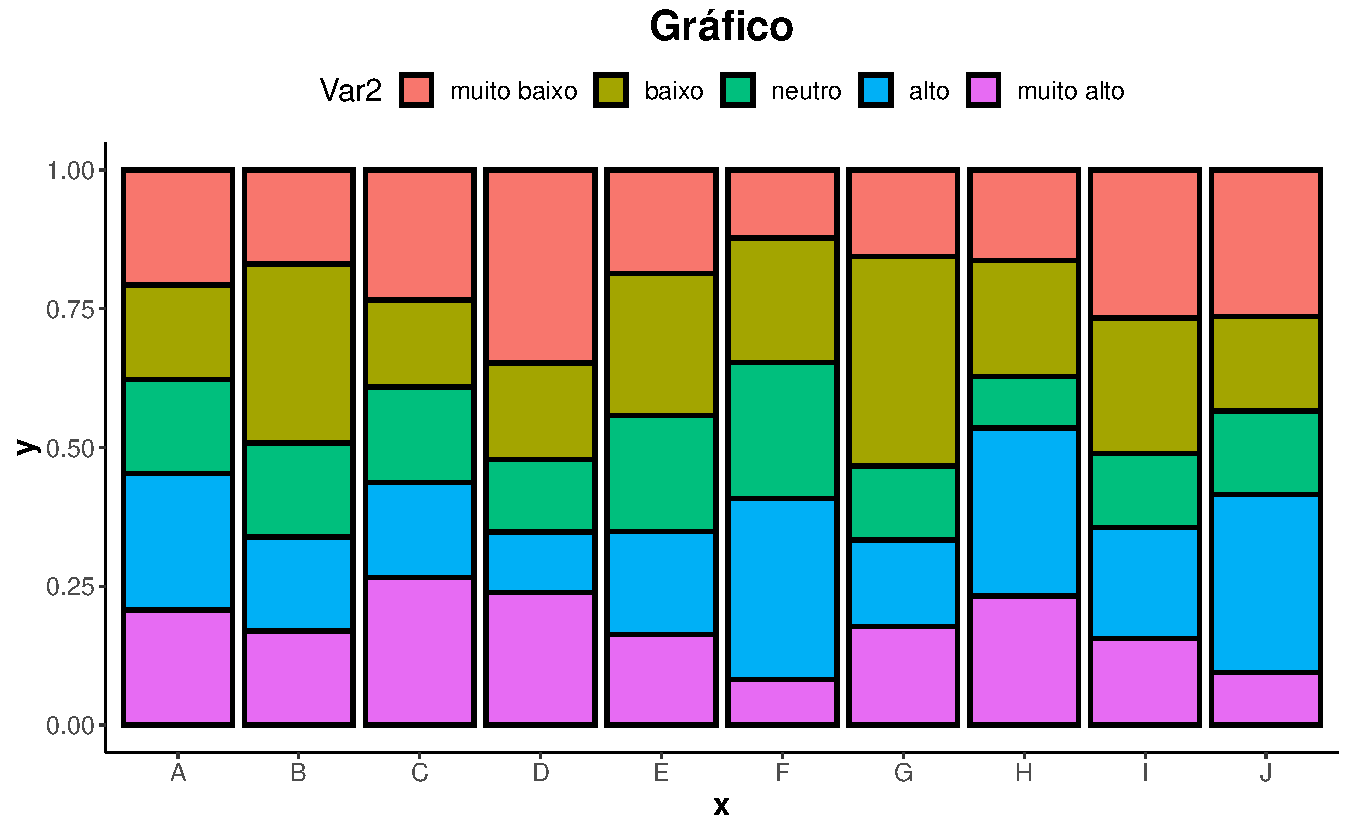
\includegraphics[width=11cm]{202-exploratoria-bivariada_files/figure-beamer/unnamed-chunk-8-1} 

}

\caption{Gráfico de barras empilhadas relativo...}\label{fig:unnamed-chunk-8}
\end{figure}
\end{frame}

\hypertarget{anuxe1lise-bivariada-para-variuxe1veis-quantitativas}{%
\section{Análise bivariada para variáveis
quantitativas}\label{anuxe1lise-bivariada-para-variuxe1veis-quantitativas}}

\begin{frame}{Análise bivariada para variáveis quantitativas}
\protect\hypertarget{anuxe1lise-bivariada-para-variuxe1veis-quantitativas-1}{}
\beginAHalfColumn

\begin{itemize}
\tightlist
\item
  Buscamos identificar \textbf{padrões} e \textbf{tendências} na análise
  das duas variáveis.

  \begin{itemize}
  \tightlist
  \item
    A medida que os valores de uma variável aumentam, a outra reduz?
  \item
    A medida que os valores de uma variável aumentam, a outra aumenta?
  \item
    A medida que os valores de uma variável aumentam, a outra se mantém
    estável?
  \end{itemize}
\end{itemize}

\endColumns
\beginAHalfColumn

\begin{itemize}
\tightlist
\item
  As principais técnicas são o \textbf{coeficiente de correlação} e o
  \textbf{diagrama de dispersão}.

  \begin{itemize}
  \tightlist
  \item
    O coeficiente é uma métrica que avalia a associação linear entre um
    par de variáveis numéricas.
  \item
    O diagrama é um gráfico de pares ordenados.
  \end{itemize}
\end{itemize}

\endColumns
\end{frame}

\begin{frame}{Coeficiente de correlação linear de Pearson}
\protect\hypertarget{coeficiente-de-correlauxe7uxe3o-linear-de-pearson}{}
\beginAHalfColumn

\begin{itemize}
\tightlist
\item
  Usado para determinar se existe \textbf{relação linear} entre
  variáveis quantitativas.

  \begin{itemize}
  \tightlist
  \item
    Assume valores entre -1 e 1.
  \item
    Se o valor é maior 0, então existe uma associação linear
    \textbf{positiva}.
  \item
    Se o valor é menor que 0, então existe uma associação linear
    \textbf{negativa}.
  \item
    Se o valor é igual a 0, então \textbf{não existe} uma associação
    linear.
  \end{itemize}
\end{itemize}

\endColumns
\beginAHalfColumn

\begin{itemize}
\tightlist
\item
  \textbf{CORRELAÇÃO NÃO IMPLICA EM CAUSALIDADE}.

  \begin{itemize}
  \tightlist
  \item
    O fato de existir uma correlação linear, seja positiva ou negativa,
    não implica que uma variável possui real influência nos desfechos da
    outra.
  \item
    Causalidade causa correlação, mas correlação não implica em
    causalidade.
  \end{itemize}
\end{itemize}

\endColumns
\end{frame}

\begin{frame}{Covariância e correlação}
\protect\hypertarget{covariuxe2ncia-e-correlauxe7uxe3o}{}
\begin{itemize}
\tightlist
\item
  A covariância entre duas variáveis \(Y_1\) e \(Y_2\) é dada por:
\end{itemize}

\[
\textrm{Cov}(y_1, y_2) = \frac{1}{n - 1}
         \displaystyle\sum_{i = 1}^{n}
         (y_{1i} - \overline{y}_1)\cdot
         (y_{2i} - \overline{y}_2).
\]

\begin{itemize}
\tightlist
\item
  A partir da covariância podemos obter a correlação, que padroniza a
  medida pelas variâncias, fazendo com que, independente das variáveis,
  sempre seja um valor entre -1 e 1.
\end{itemize}

\[
    r = \frac{\sum_{i = 1}^{n}
      (y_{1i} - \overline{y}_1)\cdot (y_{2i} - \overline{y}_2)}{
      \sqrt{\sum_{i = 1}^{n} (y_{1i} - \overline{y}_1)^2}\cdot
      \sqrt{\sum_{i = 1}^{n} (y_{2i} - \overline{y}_2)}} =
      \frac{\textrm{Cov}(y_1, y_2)}{
        \sqrt{\textrm{V}(y_1)\cdot \textrm{V}(y_2)}}.
\]
\end{frame}

\begin{frame}{Outros tipos de correlação}
\protect\hypertarget{outros-tipos-de-correlauxe7uxe3o}{}
\beginAHalfColumn

\begin{itemize}
\item
  A correlação de Pearson não serve para descrever associações que não
  sejam lineares.
\item
  Existem outros tipos de correlação que servem inclusive para variáveis
  de outros tipos.
\end{itemize}

\endColumns
\beginAHalfColumn

\begin{itemize}
\tightlist
\item
  Alguns exemplos são:

  \begin{itemize}
  \tightlist
  \item
    Correlação de Spearman.
  \item
    Correlação de Kendall.
  \item
    Ponto-bisserial.
  \end{itemize}
\end{itemize}

\endColumns
\end{frame}

\begin{frame}{Diagrama de dispersão}
\protect\hypertarget{diagrama-de-dispersuxe3o}{}
\begin{itemize}
\item
  O diagrama de dispersão é a ferramenta favorita para visualizar duas
  variáveis quantitativas.
\item
  Em um eixo são representados os valores de uma variável.
\item
  No outro eixo os valores de uma segunda variável.
\item
  Os pares ordenados são representados por pontos.
\end{itemize}
\end{frame}

\begin{frame}{Diagrama de dispersão}
\protect\hypertarget{diagrama-de-dispersuxe3o-1}{}
\begin{figure}

{\centering 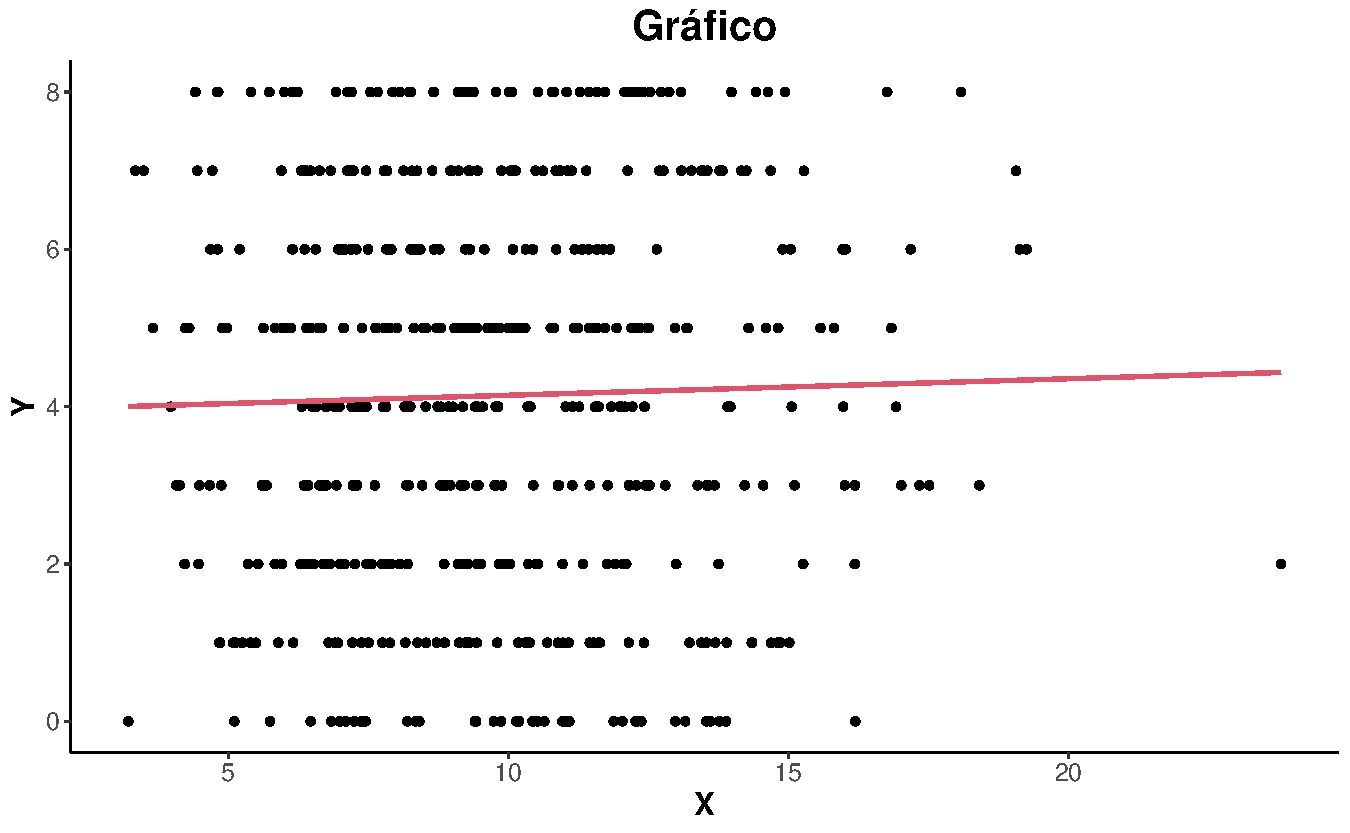
\includegraphics[width=11cm]{202-exploratoria-bivariada_files/figure-beamer/unnamed-chunk-9-1} 

}

\caption{Diagrama de dispersão...}\label{fig:unnamed-chunk-9}
\end{figure}
\end{frame}

\begin{frame}{Interpretação gráfica}
\protect\hypertarget{interpretauxe7uxe3o-gruxe1fica}{}
\begin{figure}

{\centering 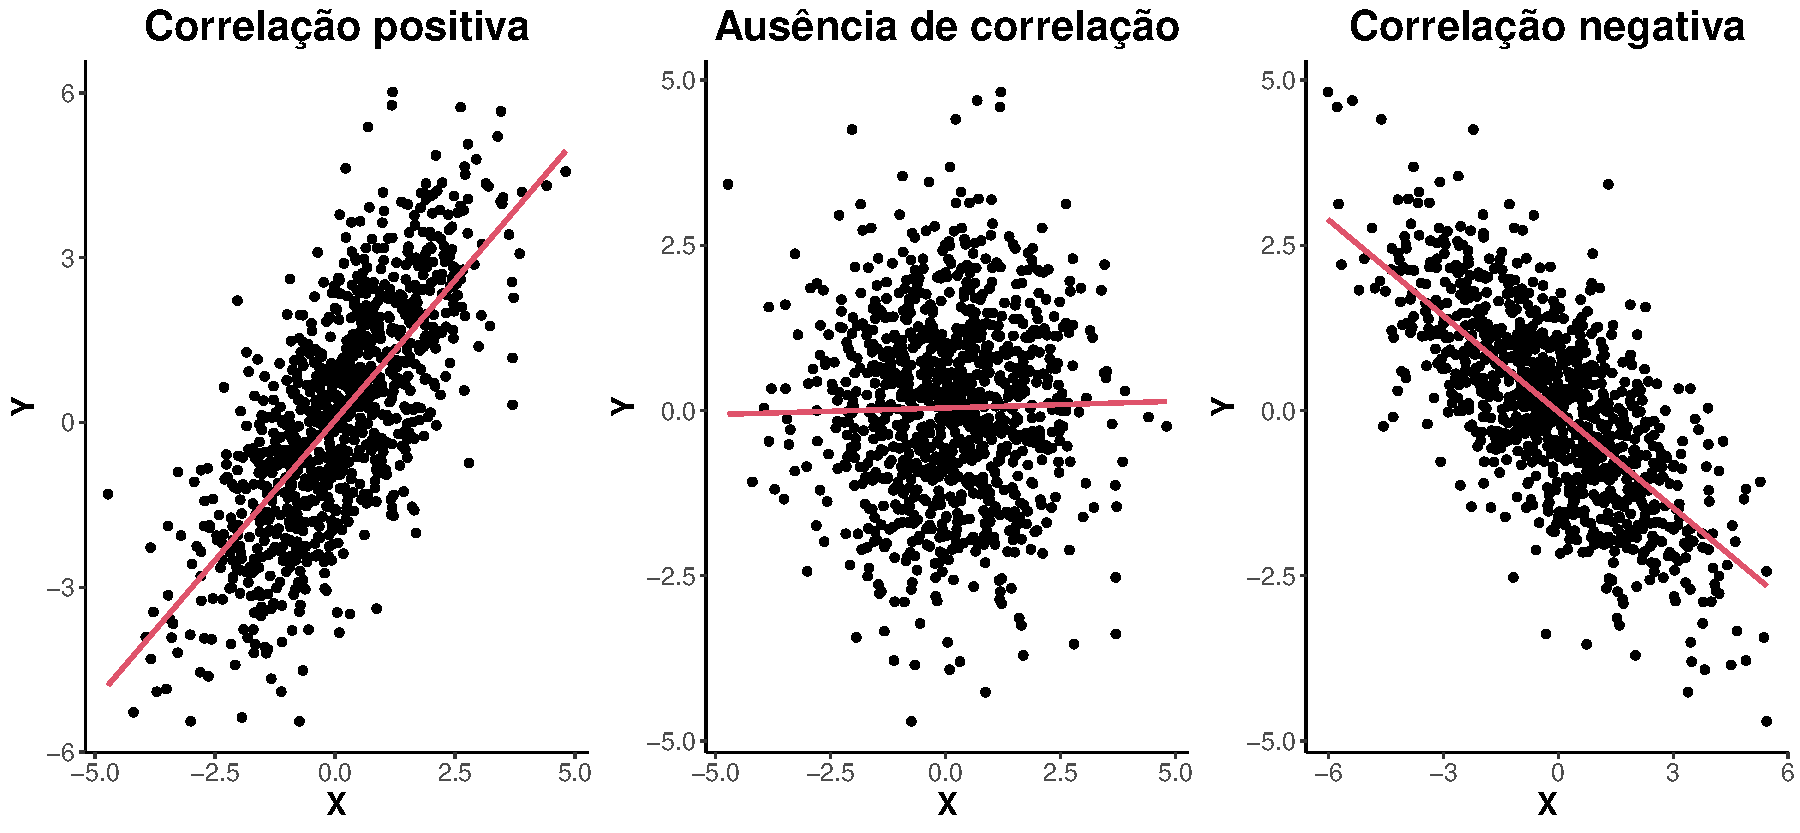
\includegraphics[width=11cm]{202-exploratoria-bivariada_files/figure-beamer/unnamed-chunk-10-1} 

}

\caption{Diagrama de dispersão...}\label{fig:unnamed-chunk-10}
\end{figure}
\end{frame}

\begin{frame}{Covariância, correlação e diagrama de dispersão}
\protect\hypertarget{covariuxe2ncia-correlauxe7uxe3o-e-diagrama-de-dispersuxe3o}{}
\textbf{Exemplo}

\begin{itemize}
\tightlist
\item
  Considere as variáveis peso (\(Y_1\)) e altura (\(Y_2\)) de um
  conjunto de 10 indivíduos.
\end{itemize}

\[Y_1: 60,09; 57,97; 54,12; 70,76; 59,74; 50,41; 58,19; 65,35; 71,18; 54,76\]

\[Y_2: 1,54; 1,62; 1,52; 1,76; 1,63; 1,52; 1,65; 1,67; 1,66; 1,57\]

\begin{itemize}
\item
  \(\overline{Y_1} = 60,26\); \(\overline{Y_2} = 1,61\).
\item
  \(Var(Y_1) = 47,8\); \(Var(Y_2) = 0,006\).
\item
  Obtenha a covariância, coeficiente de correlação e o diagrama de
  dispersão.
\end{itemize}
\end{frame}

\begin{frame}{Covariância, correlação e diagrama de dispersão}
\protect\hypertarget{covariuxe2ncia-correlauxe7uxe3o-e-diagrama-de-dispersuxe3o-1}{}
\textbf{Exemplo}

\[
\textrm{Cov}(y_1, y_2) = \frac{1}{10 - 1} \displaystyle \left \{ \left [ (60,09 - 60,26)\cdot (1,54 - 1,61) \right ] + ... + \left [ (57,76 - 60,26)\cdot (1,57 - 1,61)) \right ] \right \}
\]

\[
\textrm{Cov}(y_1, y_2) = 0,44
\]

\[
r  = \frac{0,44}{\sqrt{47,8\cdot 0,006}} = 0,82
\]
\end{frame}

\begin{frame}{Covariância, correlação e diagrama de dispersão}
\protect\hypertarget{covariuxe2ncia-correlauxe7uxe3o-e-diagrama-de-dispersuxe3o-2}{}
\textbf{Exemplo - digrama de dispersão}

\begin{figure}

{\centering 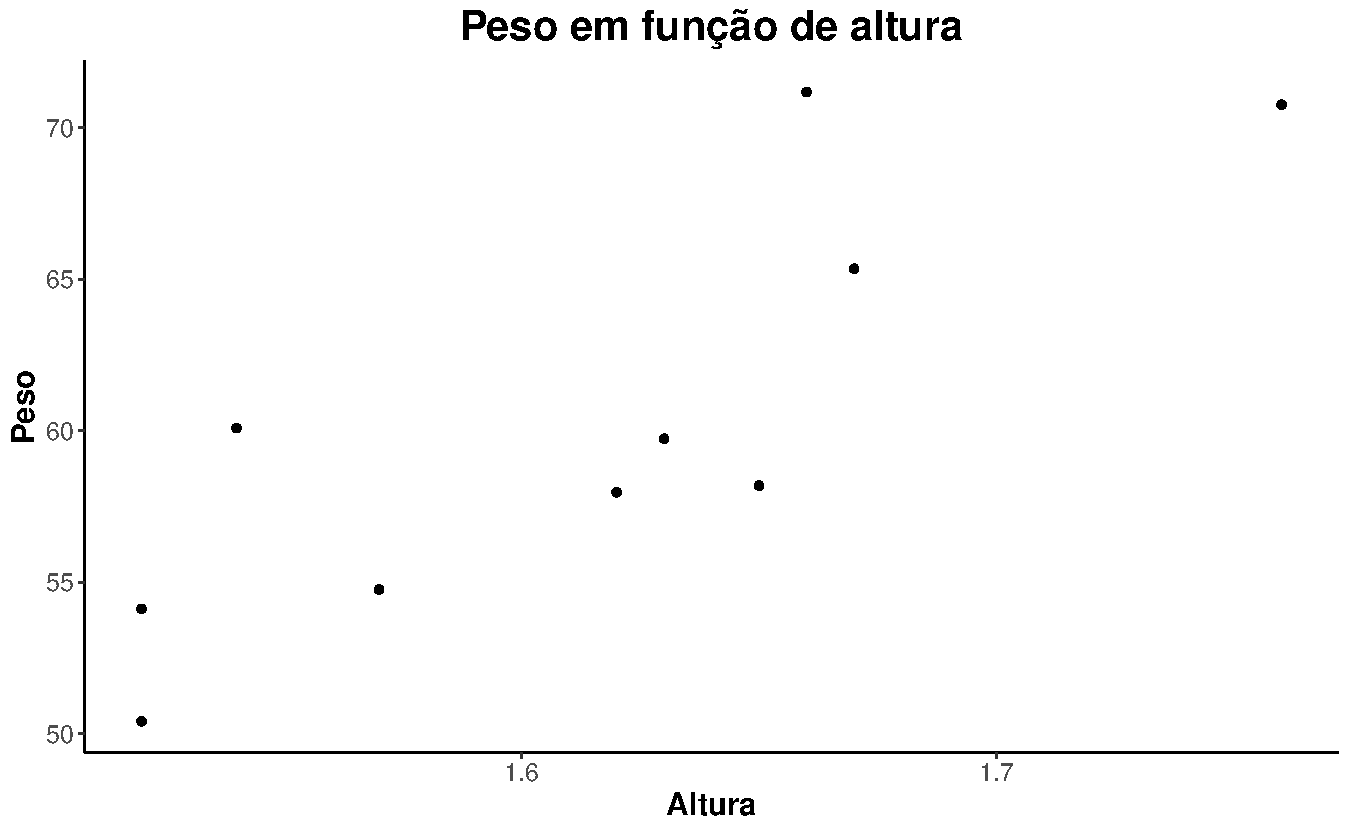
\includegraphics[width=0.65\linewidth]{202-exploratoria-bivariada_files/figure-beamer/unnamed-chunk-11-1} 

}

\caption{Diagrama de dispersão para peso e altura.}\label{fig:unnamed-chunk-11}
\end{figure}
\end{frame}

\begin{frame}{Covariância, correlação e diagrama de dispersão}
\protect\hypertarget{covariuxe2ncia-correlauxe7uxe3o-e-diagrama-de-dispersuxe3o-3}{}
\textbf{Exemplo - digrama de dispersão}

\begin{figure}

{\centering 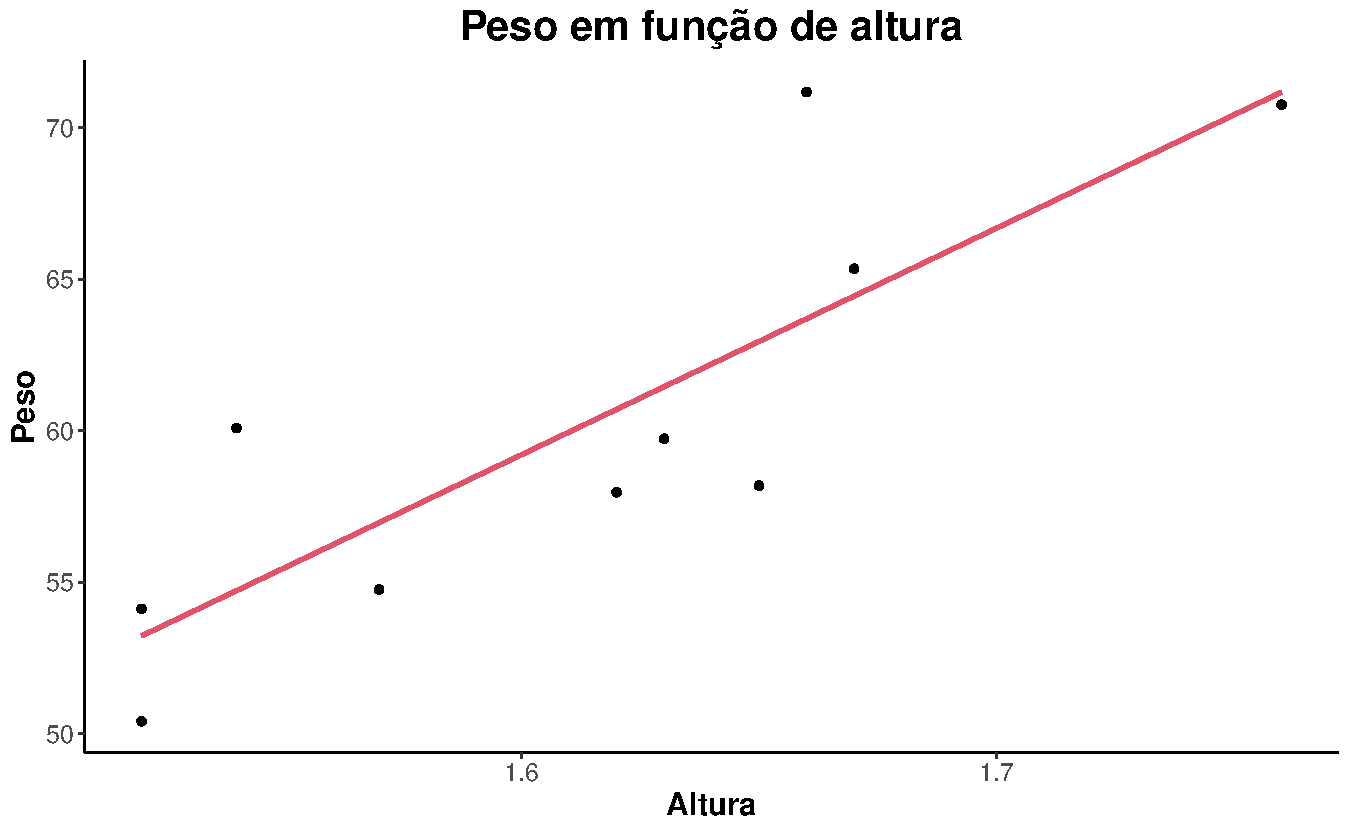
\includegraphics[width=0.65\linewidth]{202-exploratoria-bivariada_files/figure-beamer/unnamed-chunk-12-1} 

}

\caption{Diagrama de dispersão para peso e altura com linha de tendência linear.}\label{fig:unnamed-chunk-12}
\end{figure}
\end{frame}

\hypertarget{anuxe1lise-bivariada-para-uma-variuxe1vel-qualitativa-e-uma-quantitativa}{%
\section{Análise bivariada para uma variável qualitativa e uma
quantitativa}\label{anuxe1lise-bivariada-para-uma-variuxe1vel-qualitativa-e-uma-quantitativa}}

\begin{frame}{Análise bivariada para uma variável qualitativa e uma
quantitativa}
\protect\hypertarget{anuxe1lise-bivariada-para-uma-variuxe1vel-qualitativa-e-uma-quantitativa-1}{}
\begin{itemize}
\item
  Neste caso estamos interessados em avaliar se os valores da variável
  numérica estão associados com os níveis da variável categórica.
\item
  Podemos usar medidas descritivas para os valores dentro de cada um dos
  níveis da variável categórica.
\item
  Para representar graficamente esta situação podemos criar um boxplot
  da variável numérica para cada nível do fator de interesse.
\end{itemize}
\end{frame}

\begin{frame}{Tabela de medidas descritivas para níveis de um fator}
\protect\hypertarget{tabela-de-medidas-descritivas-para-nuxedveis-de-um-fator}{}
\begin{longtable}[]{@{}cccc@{}}
\caption{Tabela\ldots{}}\tabularnewline
\toprule()
nominal & Média & Mediana & Desvio padrão \\
\midrule()
\endfirsthead
\toprule()
nominal & Média & Mediana & Desvio padrão \\
\midrule()
\endhead
A & 9.84 & 9.45 & 2.85 \\
B & 9.53 & 9.37 & 3.28 \\
C & 9.22 & 8.91 & 2.83 \\
D & 9.65 & 9.64 & 2.48 \\
E & 9.97 & 9.79 & 2.99 \\
F & 10.05 & 9.20 & 3.48 \\
G & 9.96 & 10.35 & 2.91 \\
H & 10.44 & 10.44 & 3.71 \\
I & 9.00 & 9.04 & 3.29 \\
J & 9.97 & 9.32 & 3.41 \\
\bottomrule()
\end{longtable}
\end{frame}

\begin{frame}{Box-plot para níveis de um fator}
\protect\hypertarget{box-plot-para-nuxedveis-de-um-fator}{}
\begin{figure}

{\centering 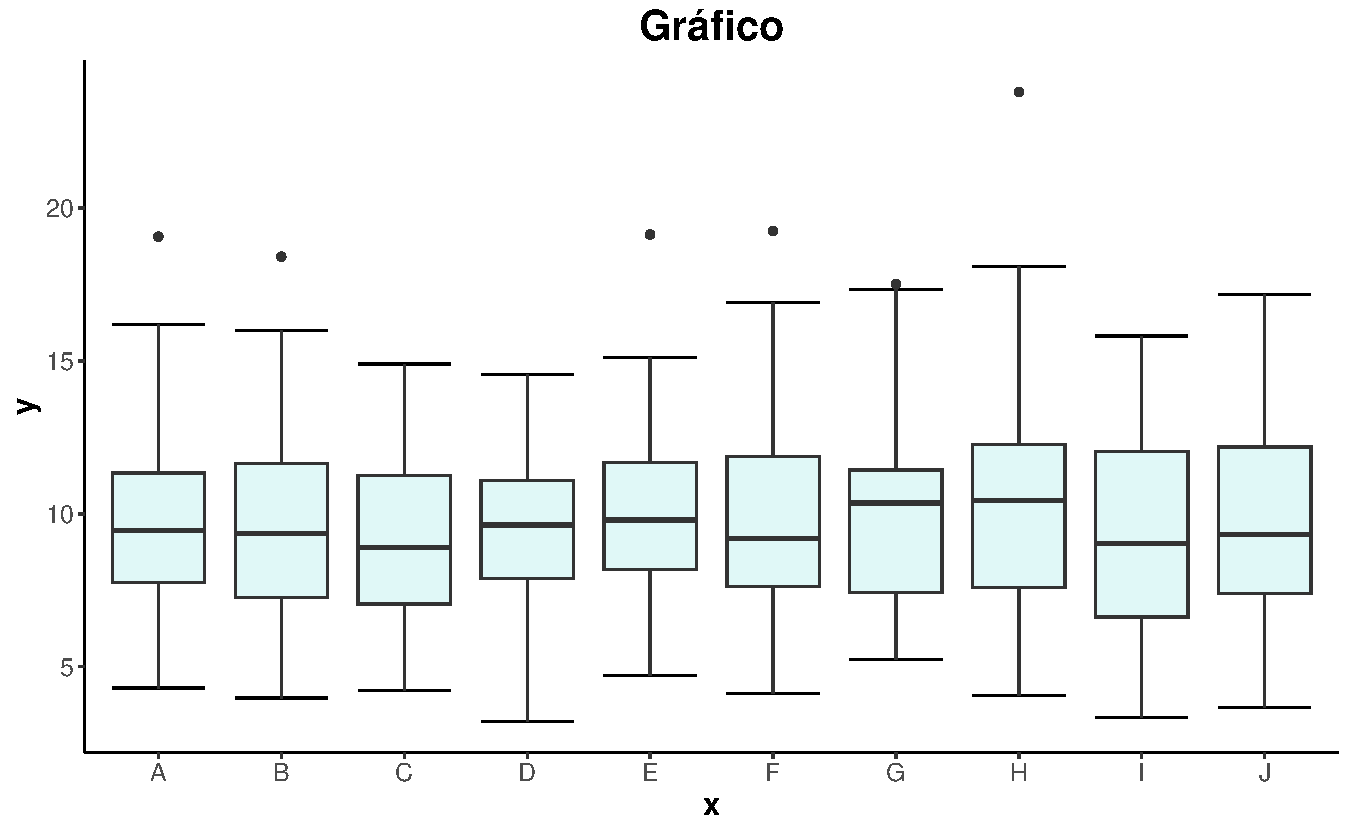
\includegraphics[width=11cm]{202-exploratoria-bivariada_files/figure-beamer/unnamed-chunk-14-1} 

}

\caption{box-plot para}\label{fig:unnamed-chunk-14}
\end{figure}
\end{frame}

\hypertarget{outros-tipos-de-gruxe1ficos-e-anuxe1lises}{%
\section{Outros tipos de gráficos e
análises}\label{outros-tipos-de-gruxe1ficos-e-anuxe1lises}}

\begin{frame}{Outros tipos de gráficos e análises}
\protect\hypertarget{outros-tipos-de-gruxe1ficos-e-anuxe1lises-1}{}
\beginAHalfColumn

\begin{itemize}
\item
  Vimos as alternativas usuais para representação e análise de variáveis
  quantitativas e qualitativas.
\item
  Contudo existem diversas situações particulares que exigem análises
  específicas.
\end{itemize}

\endColumns
\beginAHalfColumn

\begin{itemize}
\item
  Algumas casos são: mapas, séries temporais, gráficos de perfil, nuvens
  de palavras.
\item
  Também é possível trabalhar com gráficos que representam mais de duas
  variáveis ao mesmo tempo.
\item
  Outra possibilidade é combinar gráficos.
\end{itemize}

\endColumns
\end{frame}

\begin{frame}{}
\protect\hypertarget{section}{}
\beginAHalfColumn

\textbf{O que foi visto:}

\begin{itemize}
\tightlist
\item
  Análises bivariadas.

  \begin{itemize}
  \tightlist
  \item
    Qualitativa x qualitativa.
  \item
    Quantitativa x quantitativa.
  \item
    Quantitativa x qualitativa.
  \end{itemize}
\end{itemize}

\endColumns
\beginAHalfColumn

\textbf{Próximos assuntos:}

\begin{itemize}
\tightlist
\item
  Introdução à probabilidades.
\end{itemize}

\endColumns
\end{frame}

\end{document}
